%==============================================================================
% Figure: Dimensional Tower (Hierarchy)
% Purpose: Vertical tower showing dimensional scales from Planck to observable
% Chapter: Ch20 - Dimensional Reconciliation
% Type: Conceptual
%==============================================================================

\begin{figure}[htbp]
  \centering
  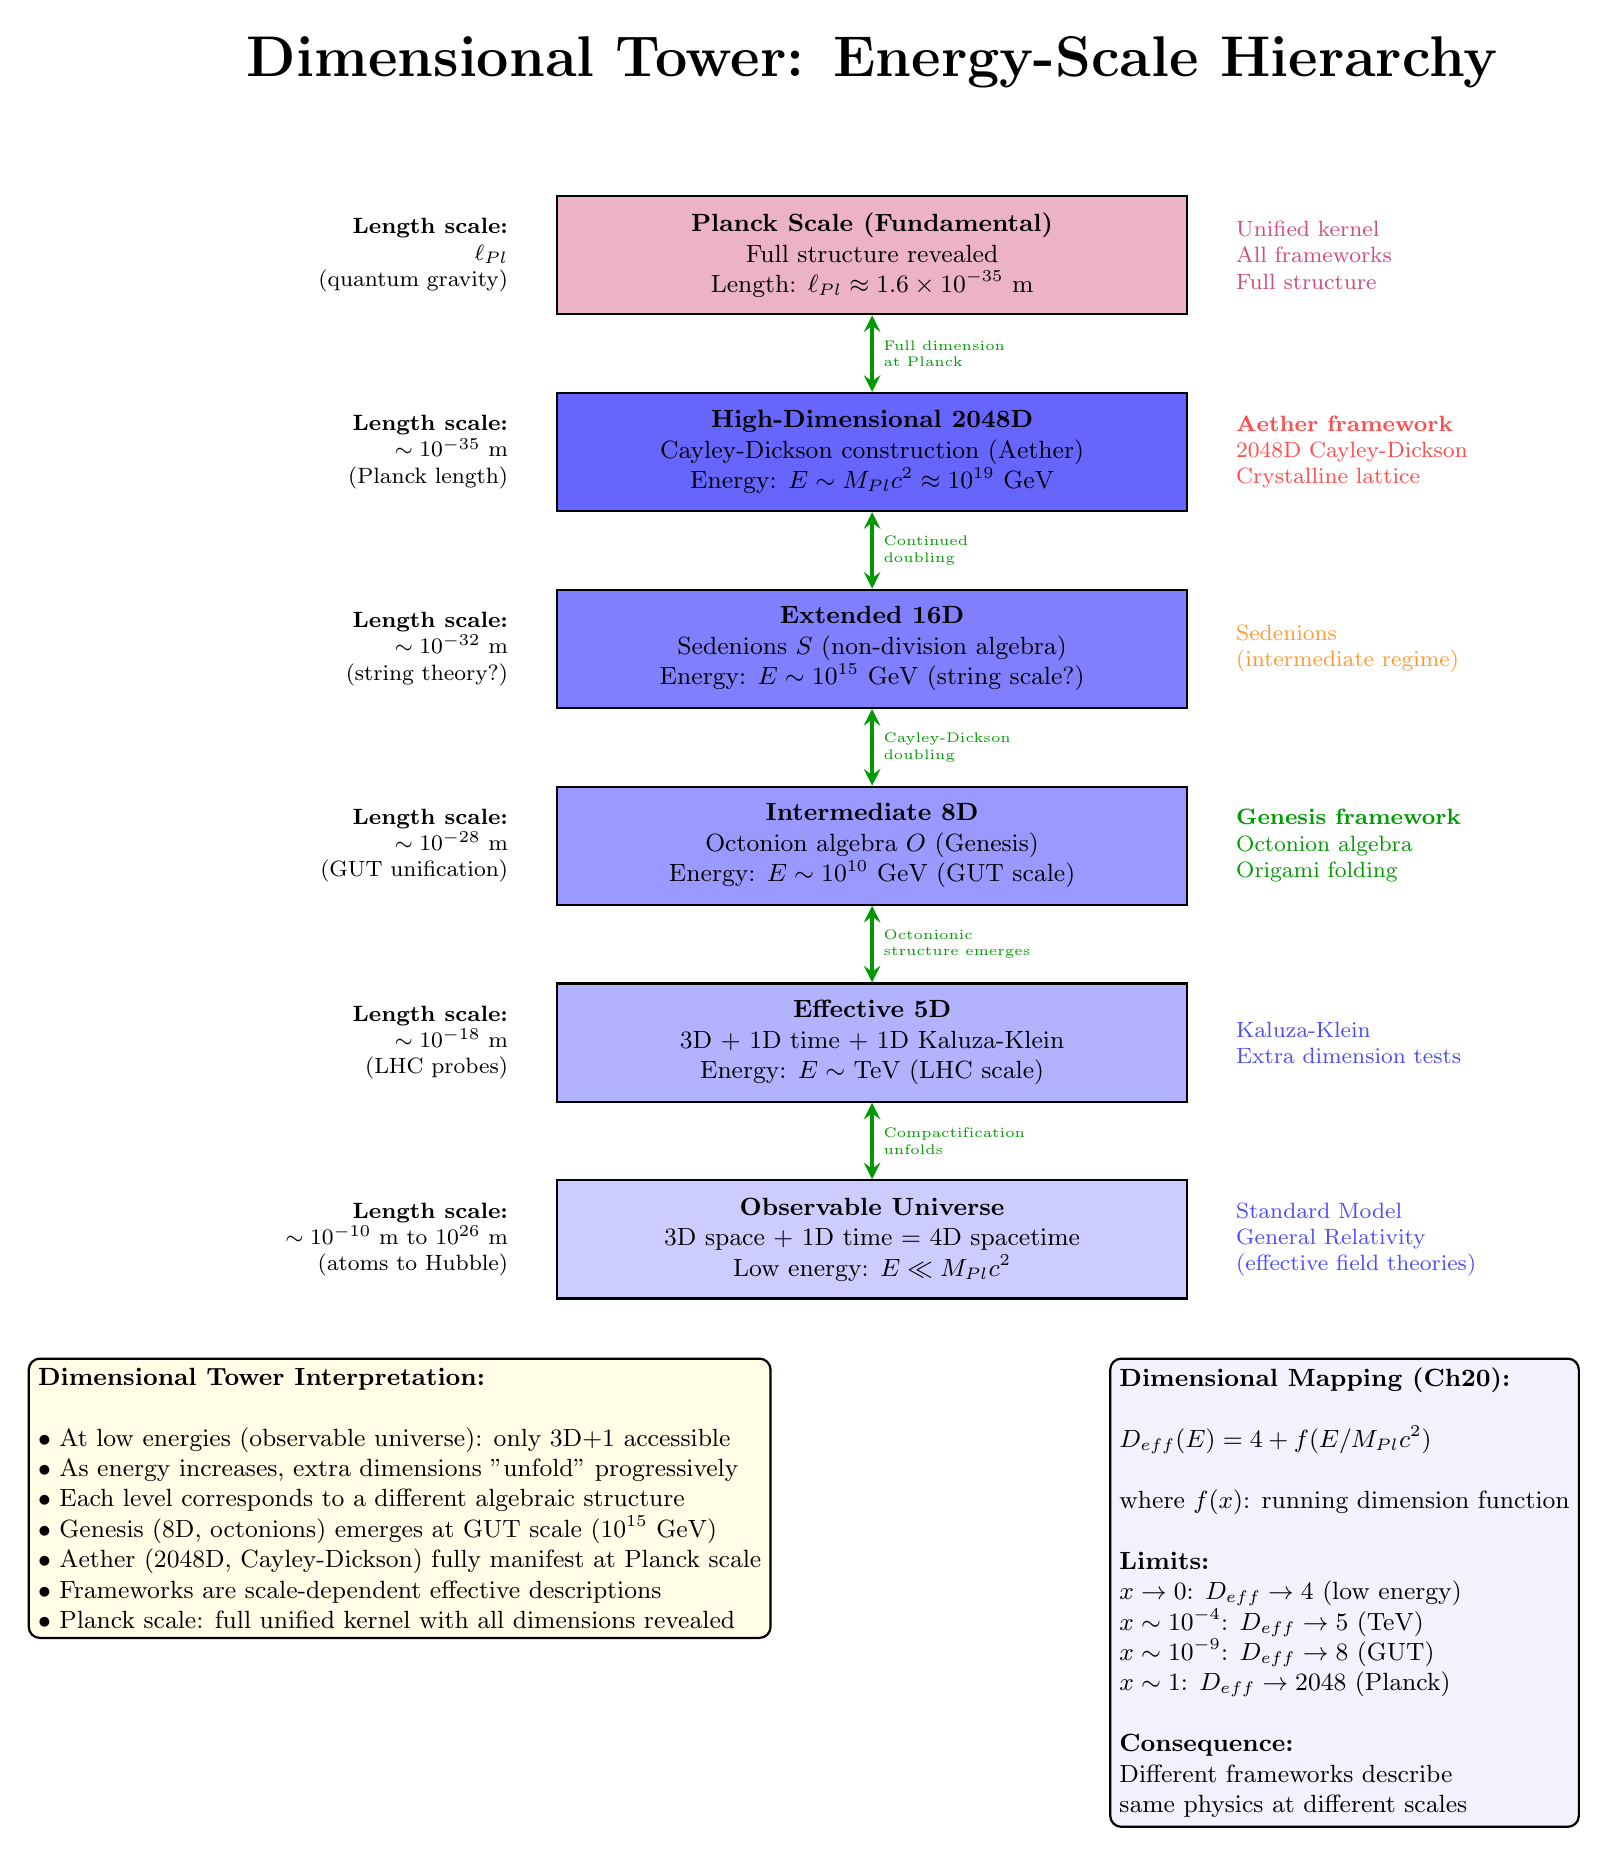
\begin{tikzpicture}[
    scale=1.0,
    level/.style={rectangle, draw=black, thick, minimum width=8cm, minimum height=1.5cm, align=center, font=\small},
    arrow/.style={<->, >=stealth, ultra thick}
  ]

    %========== Dimensional Levels (bottom to top) ==========

    % Level 1: Observable 3D+1
    \node[level, fill=blue!20] (obs) at (0, 0) {
      \textbf{Observable Universe} \\
      3D space + 1D time = 4D spacetime \\
      Low energy: $E \ll M_{\text{Pl}}c^2$
    };

    % Level 2: Effective 5D
    \node[level, fill=blue!30] (eff5) at (0, 2.5) {
      \textbf{Effective 5D} \\
      3D + 1D time + 1D Kaluza-Klein \\
      Energy: $E \sim$ TeV (LHC scale)
    };

    % Level 3: Intermediate 8D
    \node[level, fill=blue!40] (int8) at (0, 5.0) {
      \textbf{Intermediate 8D} \\
      Octonion algebra $\mathbb{O}$ (Genesis) \\
      Energy: $E \sim 10^{10}$ GeV (GUT scale)
    };

    % Level 4: Extended 16D
    \node[level, fill=blue!50] (ext16) at (0, 7.5) {
      \textbf{Extended 16D} \\
      Sedenions $\mathbb{S}$ (non-division algebra) \\
      Energy: $E \sim 10^{15}$ GeV (string scale?)
    };

    % Level 5: High-dimensional 2048D
    \node[level, fill=blue!60] (high2048) at (0, 10.0) {
      \textbf{High-Dimensional 2048D} \\
      Cayley-Dickson construction (Aether) \\
      Energy: $E \sim M_{\text{Pl}}c^2 \approx 10^{19}$ GeV
    };

    % Level 6: Planck-scale fundamental
    \node[level, fill=purple!30] (planck) at (0, 12.5) {
      \textbf{Planck Scale (Fundamental)} \\
      Full structure revealed \\
      Length: $\ell_{\text{Pl}} \approx 1.6 \times 10^{-35}$ m
    };

    %========== Arrows showing hierarchy ==========
    \draw[arrow, green!60!black] (obs.north) -- (eff5.south)
      node[midway, right, font=\tiny, align=left] {Compactification\\unfolds};
    \draw[arrow, green!60!black] (eff5.north) -- (int8.south)
      node[midway, right, font=\tiny, align=left] {Octonionic\\structure emerges};
    \draw[arrow, green!60!black] (int8.north) -- (ext16.south)
      node[midway, right, font=\tiny, align=left] {Cayley-Dickson\\doubling};
    \draw[arrow, green!60!black] (ext16.north) -- (high2048.south)
      node[midway, right, font=\tiny, align=left] {Continued\\doubling};
    \draw[arrow, green!60!black] (high2048.north) -- (planck.south)
      node[midway, right, font=\tiny, align=left] {Full dimension\\at Planck};

    %========== Side annotations: Scale labels ==========
    \node[anchor=east, align=right, font=\footnotesize] at (-4.5, 0) {
      \textbf{Length scale:} \\
      $\sim 10^{-10}$ m to $10^{26}$ m \\
      (atoms to Hubble)
    };

    \node[anchor=east, align=right, font=\footnotesize] at (-4.5, 2.5) {
      \textbf{Length scale:} \\
      $\sim 10^{-18}$ m \\
      (LHC probes)
    };

    \node[anchor=east, align=right, font=\footnotesize] at (-4.5, 5.0) {
      \textbf{Length scale:} \\
      $\sim 10^{-28}$ m \\
      (GUT unification)
    };

    \node[anchor=east, align=right, font=\footnotesize] at (-4.5, 7.5) {
      \textbf{Length scale:} \\
      $\sim 10^{-32}$ m \\
      (string theory?)
    };

    \node[anchor=east, align=right, font=\footnotesize] at (-4.5, 10.0) {
      \textbf{Length scale:} \\
      $\sim 10^{-35}$ m \\
      (Planck length)
    };

    \node[anchor=east, align=right, font=\footnotesize] at (-4.5, 12.5) {
      \textbf{Length scale:} \\
      $\ell_{\text{Pl}}$ \\
      (quantum gravity)
    };

    %========== Framework associations ==========
    \node[anchor=west, align=left, font=\footnotesize, text=blue!70] at (4.5, 0) {
      Standard Model \\
      General Relativity \\
      (effective field theories)
    };

    \node[anchor=west, align=left, font=\footnotesize, text=blue!70] at (4.5, 2.5) {
      Kaluza-Klein \\
      Extra dimension tests
    };

    \node[anchor=west, align=left, font=\footnotesize, text=green!60!black] at (4.5, 5.0) {
      \textbf{Genesis framework} \\
      Octonion algebra \\
      Origami folding
    };

    \node[anchor=west, align=left, font=\footnotesize, text=orange!80] at (4.5, 7.5) {
      Sedenions \\
      (intermediate regime)
    };

    \node[anchor=west, align=left, font=\footnotesize, text=red!70] at (4.5, 10.0) {
      \textbf{Aether framework} \\
      2048D Cayley-Dickson \\
      Crystalline lattice
    };

    \node[anchor=west, align=left, font=\footnotesize, text=purple!70] at (4.5, 12.5) {
      Unified kernel \\
      All frameworks \\
      Full structure
    };

    %========== Bottom explanation box ==========
    \node[anchor=north, align=left, font=\small, draw=black, fill=yellow!10, rounded corners, thick]
      at (-6, -1.5) {
      \textbf{Dimensional Tower Interpretation:} \\
      \\
      $\bullet$ At low energies (observable universe): only 3D+1 accessible \\
      $\bullet$ As energy increases, extra dimensions "unfold" progressively \\
      $\bullet$ Each level corresponds to a different algebraic structure \\
      $\bullet$ Genesis (8D, octonions) emerges at GUT scale ($10^{15}$ GeV) \\
      $\bullet$ Aether (2048D, Cayley-Dickson) fully manifest at Planck scale \\
      $\bullet$ Frameworks are scale-dependent effective descriptions \\
      $\bullet$ Planck scale: full unified kernel with all dimensions revealed
    };

    \node[anchor=north, align=left, font=\small, draw=black, fill=blue!5, rounded corners, thick]
      at (6, -1.5) {
      \textbf{Dimensional Mapping (Ch20):} \\
      \\
      $D_{\text{eff}}(E) = 4 + f(E/M_{\text{Pl}}c^2)$ \\
      \\
      where $f(x)$: running dimension function \\
      \\
      \textbf{Limits:} \\
      $x \to 0$: $D_{\text{eff}} \to 4$ (low energy) \\
      $x \sim 10^{-4}$: $D_{\text{eff}} \to 5$ (TeV) \\
      $x \sim 10^{-9}$: $D_{\text{eff}} \to 8$ (GUT) \\
      $x \sim 1$: $D_{\text{eff}} \to 2048$ (Planck) \\
      \\
      \textbf{Consequence:} \\
      Different frameworks describe \\
      same physics at different scales
    };

    %========== Title ==========
    \node[anchor=south, font=\huge\bfseries] at (0, 14.5) {Dimensional Tower: Energy-Scale Hierarchy};

  \end{tikzpicture}
  \caption{Vertical dimensional tower showing the hierarchy of effective dimensions as a function
    of energy scale, reconciling the different dimensionalities of Aether (2048D), Genesis (8D),
    and observable spacetime (4D). At low energies (bottom, blue), only 3 spatial dimensions plus
    time are accessible---the regime of Standard Model and General Relativity. As energy increases,
    compactified dimensions progressively "unfold": at TeV scale (LHC), a 5th Kaluza-Klein dimension
    may become visible; at GUT scale ($\sim 10^{15}$ GeV), the full octonion structure of Genesis
    (8D) emerges; at intermediate string-scale energies, sedenions (16D) appear; approaching Planck
    energy ($\sim 10^{19}$ GeV), the Aether framework's full 2048D Cayley-Dickson algebra becomes
    manifest. At the Planck scale (top, purple), all frameworks converge in the unified kernel with
    full dimensional structure revealed. The left column shows corresponding length scales (from
    Hubble radius $\sim 10^{26}$ m down to Planck length $\ell_{\text{Pl}} \sim 10^{-35}$ m), and
    the right column associates frameworks with each level. This tower resolves the apparent conflict
    between frameworks: they are scale-dependent effective descriptions of the same underlying physics,
    with effective dimension $D_{\text{eff}}(E)$ running from 4 to 2048 as energy increases from
    zero to Planck scale (Ch20 provides the explicit mapping function). Experimental probes at
    different energies access different levels of this tower.}
  \label{fig:dimensional-tower}
\end{figure}
